\documentclass[10pt,letterpaper]{article}
\usepackage[margin=0.45in]{geometry}
\usepackage[T1]{fontenc}
\usepackage{lmodern,graphicx,xcolor,inconsolata}
\usepackage[hidelinks]{hyperref}
\pagestyle{empty}
\setlength{\parindent}{0pt}
\setlength{\parskip}{5pt}
\renewcommand{\familydefault}{\sfdefault}
% Shared color roles, generated by scripts/build.py.
\definecolor{frkApplication}{HTML}{075985}
\definecolor{frkSupervision}{HTML}{92400E}
\definecolor{frkSecondary}{HTML}{52525B}

\newcommand{\guideurl}{https://github.com/rduncangt/frk-management/blob/pan-head-screw-qr-pilot/parts/11416567700/README.md}
\begin{document}
\begin{minipage}[c]{0.83\linewidth}
  % Logo source: https://teamrubiconusa.org/ (TRDR_logo_rgb.png).
  \begin{minipage}[c]{1.08in}
    
\includegraphics[width=\linewidth]{../images/team-rubicon-logo.png}
  \end{minipage}\hspace{0.16in}%
  \begin{minipage}[c]{2.25in}
    {\fontsize{8}{10}\selectfont\color{frkSecondary} FIELD REPAIR KIT --- PART REFERENCE}
  \end{minipage}\par
  {\fontsize{21}{24}\selectfont\bfseries Chain catcher\par}
  {\fontsize{18}{21}\selectfont\ttfamily\bfseries 1141 656 7700\par}
  {\small\color{frkSecondary} Bin \textcolor{black}{\textbf{A8}} \enspace | \enspace \textcolor{black}{\textbf{3}} spares per kit \enspace | \enspace \textcolor{frkSupervision}{\textbf{AS1}} supervision}
\end{minipage}\hfill
\begin{minipage}[c]{0.14\linewidth}
  \centering
  \href{\guideurl}{
\includegraphics[width=0.82in]{images/qr.png}}\par
  {\scriptsize\color{frkSecondary} Online guide}
\end{minipage}
\par\smallskip\hrule\medskip
{\large\bfseries\color{frkApplication} MS 261 --- chain catcher mounting\par}
Mounts to the clutch-side crankcase with pan head self-tapping screw
\textbf{9074 477 4438} (IS-P6$\times$30; item 40).\par
\textbf{Item 39 \enspace | \enspace Qty fitted: 1}\par
\medskip
\begin{center}
  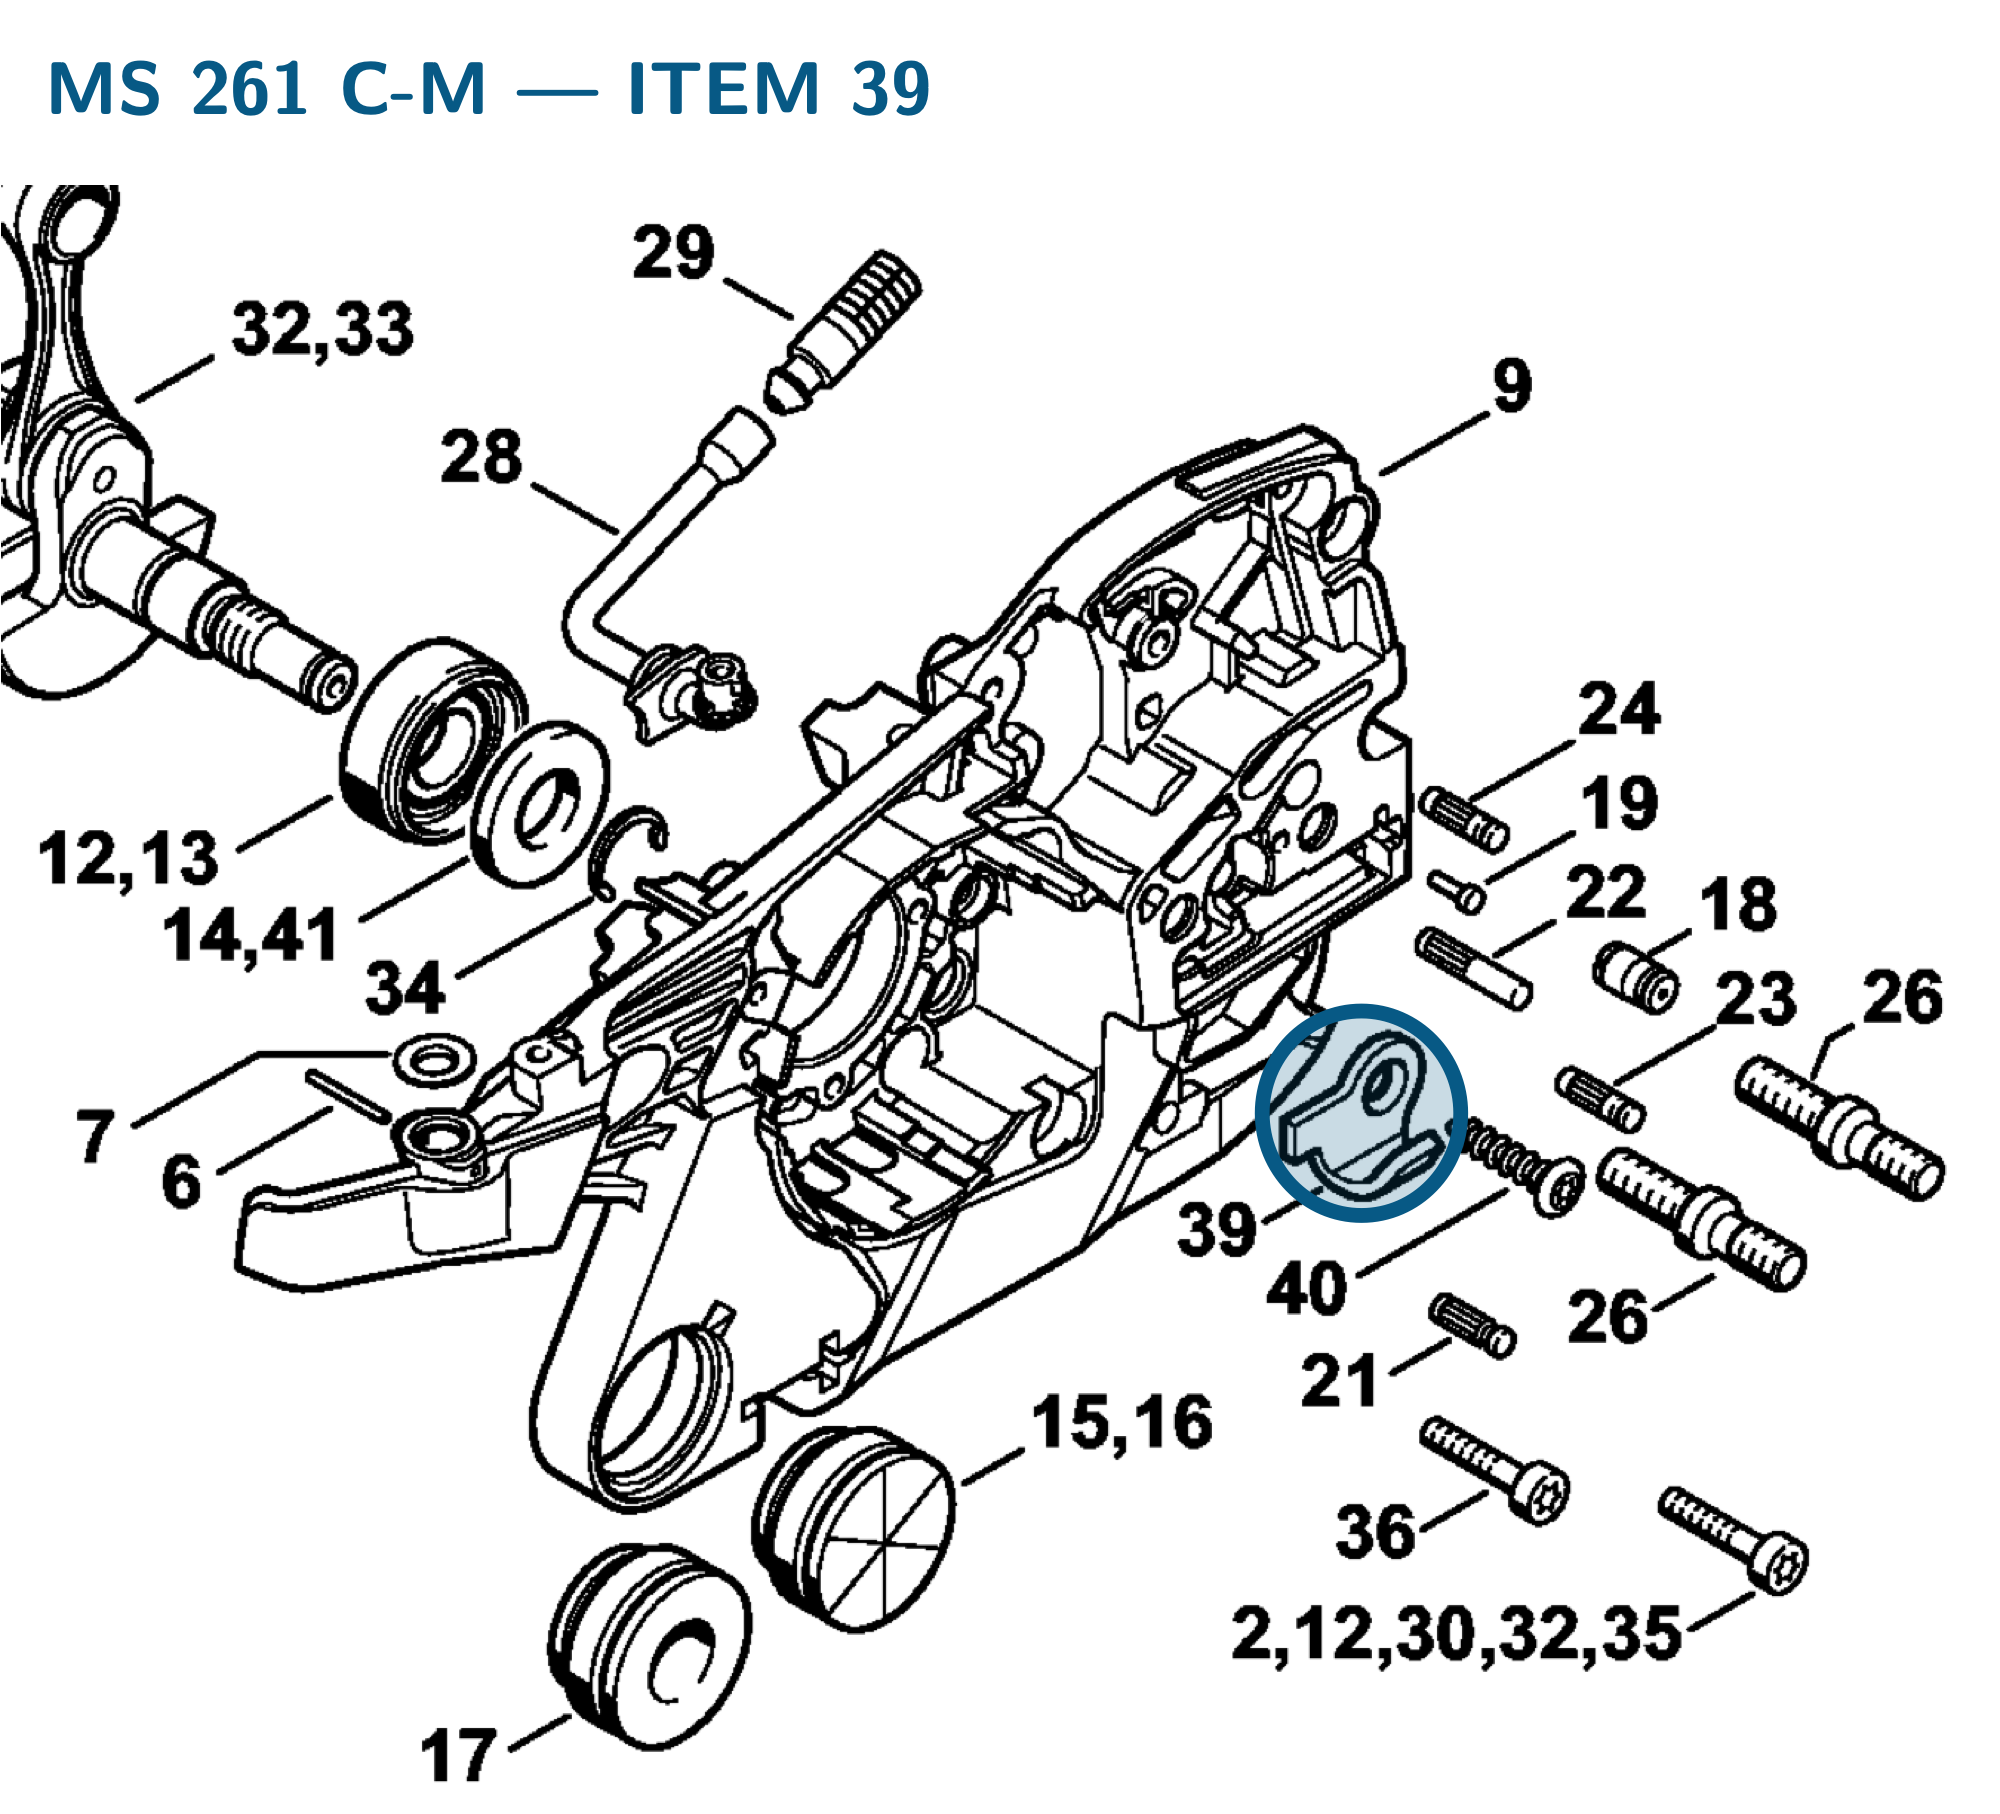
\includegraphics[width=5.3in,height=4.85in,keepaspectratio]{images/ms261-chain-catcher.png}
\end{center}
{\footnotesize\color{frkSecondary}
  MS 261 C-M spare-parts list, 10/02/2023.\newline
  Crankcase; PDF drawing p.\ 3, parts table p.\ 5.\par
}
\smallskip\hrule\smallskip
{\footnotesize\color{frkSecondary}
  Drawing \textcopyright\ ANDREAS STIHL AG \& Co. KG. Not to scale. \hfill 2026-09-27
}
\end{document}
